%!TEX root = ../thesis.tex

\cleardoublepage
\chapter{Introduction}

\label{cha:introduction}

%%=========================================
\section{Motivation and Problem Description}
\label{sec:motivation}

One of the aims for the fifth generation of mobile networks (5G) and it's successors is a greater diversification of the classes of service they offer. As the use cases for these networks evolve, there is a greater need for quality of service (QoS) tailored to each use case. For example, Industrial Internet of Things (IIoT) applications have stringent requirements on latency, jitter, and reliability. Supporting these kinds of classes of service can be a challenge for mobile network operators (MNOs) and will require novel approaches to familiar problems, such as backhaul.

As there are more heterogeneous edge deployments and more campus networks, backhaul becomes more challenging, since many sites may not have access to optical fibre, and may be forced into using other solutions such as satellite links, mmWave backhaul, or the connections of their Internet Service Provider (ISP). Providing the kind of deterministic quality of service that these sites may require can be a difficult challenge.

Particularly with the rise of satellite backhaul options, fuelled by the new space race, remote deployments may choose to integrate satellite backhaul because fibre is infeasible in their location or its roll-out is too slow. When these connections are added to the site of a deployment it is usually in addition to a pre-existing one. Thus network operators could choose to utilize both the new and the old backhaul connection at the same time, in order to utilize the different qualities of the backhaul links. This bears the question whether multipathing could be used to provide deterministic backhaul by intelligently selecting on which links to forward packets. This approach bears similarity to multihoming as well as to multi-path routing in Wireless Sensor Networks (WSNs), and can take inspiration from the substantial body of research in these fields which already exists. That research has demonstrated that using multiple links or paths simultaneously can improve QoS \cite{akella2003measurement, tao2005improving, habib2007improving, goldenberg2004optimizing, huang2008multiconstrained, akella2008performance}, and prompts the question whether something similar could be done to address backhaul in 5G campus networks.


%\LTXtable{\textwidth}{tab/scenario1_sensor}

%%=========================================
\section{Target}
\label{sec:target}

The goal of this thesis is to design and provide an implementation of a Wide Area Network connector (WAN Connector), that can be placed at the ingress and egress point of two locations. It should then utilize multipathing in order to provide deterministic backhaul between the two sites. The performance of this approach will then be quantitatively analyzed in experiments.

\begin{figure}[h]
    \centering
        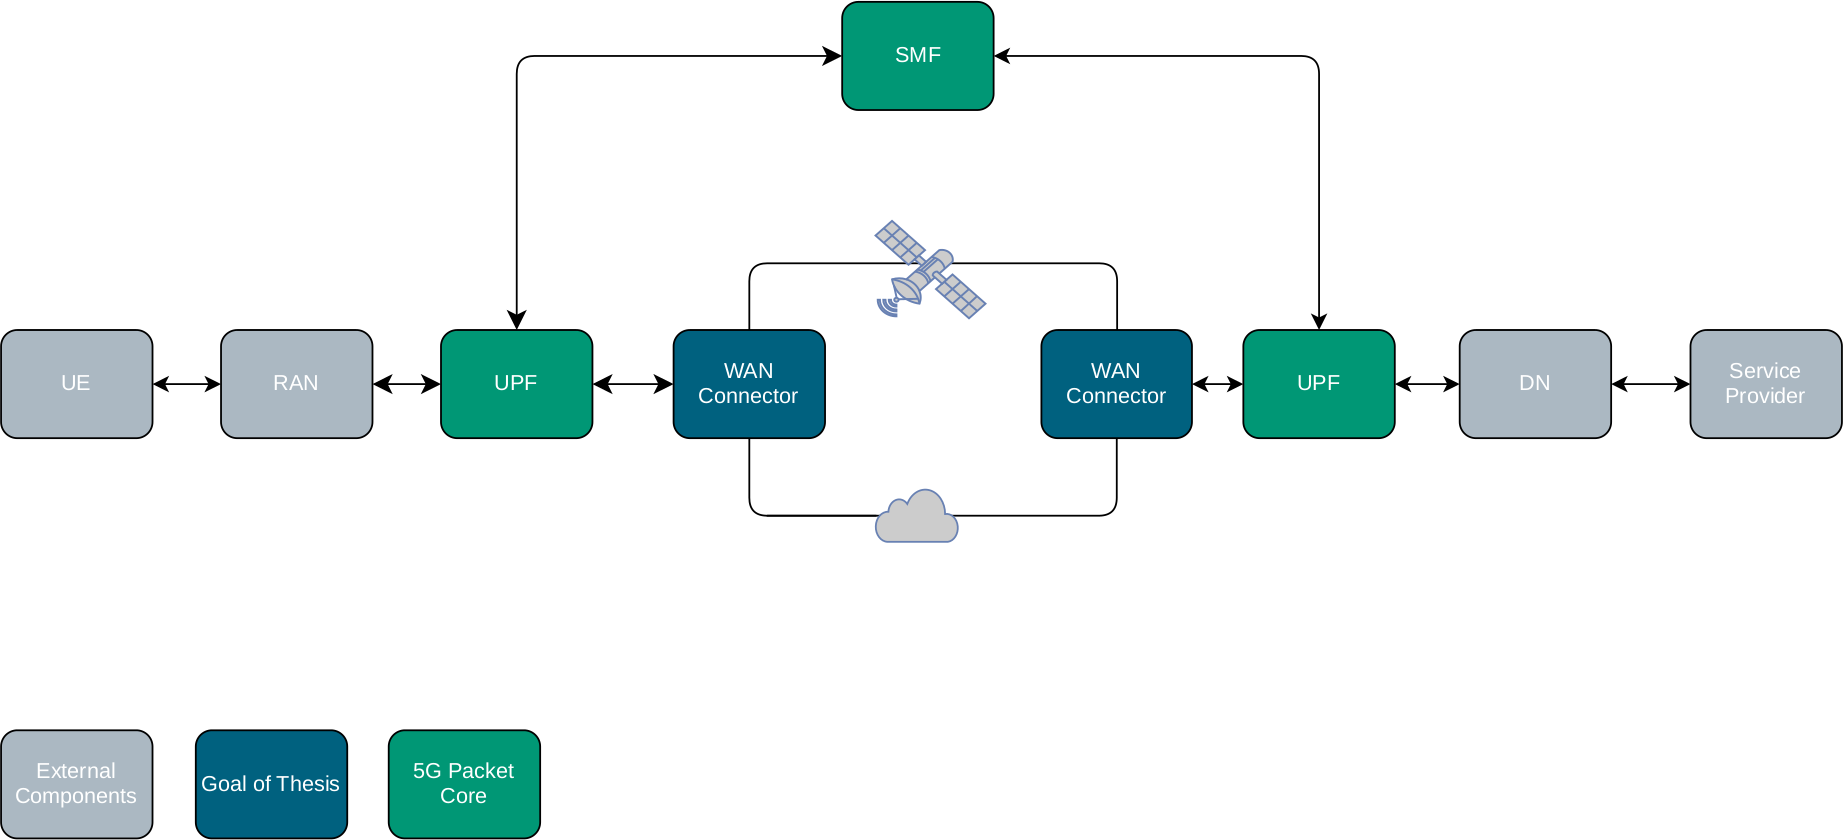
\includegraphics[width=\textwidth]{fig/telco-use-case-2.png}
        \caption{5G Deployment with 2 UPFs}
        \label{fig:telco}
\end{figure}

Looking at Figure \ref{fig:telco} we can see how this is envisioned to work. WAN Connectors are deployed both in the geographically distributed 5G campus network, which has more than one egress link, and in the core. Then, using the multiple outgoing links, they backhaul traffic to the other site, while respecting the traffic's QoS requirements. This can be especially beneficial for critical applications (e.g. at industrial sites), which are in locations that do not have access to optical fibre for backhaul.

For a 5G deployment the proposed WAN Connector could be deployed in between two User Plane Functions (UPF's) , in order to provide deterministic backhaul. The architecture for such a deployment is shown in Figure \ref{fig:telco}. Further, the on-site UPF is not a strict requirement; it is also feasible to connect the RAN directly to the WAN Connector.


%%=========================================
\section{Scope}
\label{sec:scope}

While a high level design will be presented, and a first implementation will be tested, this implementation will not be industry grade and should not be judged next to commercial packet processing products.  Furthermore, an explicit specification for the format of communication with the 5G Core's control plane is largely beyond the scope of this thesis. Although an interface to the 5G Core's Session Management Function (SMF) will be assumed, it is not specified nor implemented. By some means the flows and their requirements must be communicated to the WAN Connector over the control plane, however an exact description of the data formats used in this communication will not occur. The user plane interface to the WAN Connector is not described either. However, the WAN Connector may be able to act in a fashion which is opaque to the user plane component with which it is interacting (RAN or UPF). The WAN Connector can bridge both the N3 or N9 reference points. The user plane traffic is simply forwarded to the WAN Connector and backhauled to the second WAN Connector, which reintroduces it into the other user plane component. No part of the user plane needs to be aware that the WAN Connector is sitting in the middle.

Lastly, in the process of investigating multipathing for deterministic backhaul, this thesis will not test the WAN Connector in a real deployment at a remote site. Additionally, the tests will not instantiate a full 5G Core network for the tests, and will not feature UPF's, a RAN, nor UE's (like in graphic number \ref{fig:telco}).

%=======================
\section{Structure}

This thesis will follow a 7 chapter structure. This section concludes the introduction chapter, what follows will be one chapter to provide both basic background information as well as to highlight the existing literature which is of relevance to the problem statement. Next will be the requirements, design, and implementation chapters. Then, the evaluation chapter will analyze the WAN Connector's performance. The conclusion chapter will review the relevant findings, the successes and failures of the approach, how to improve on it, and lastly the possibilities for future research in this area.

%%=========================================

%%% include all uncited works that we still want to cite

\nocite{tsai2006review}
\nocite{rodriguez2004mar}
\nocite{tarique2009survey}
\nocite{tao2004application}
\nocite{zand2012wireless}
\nocite{li2016multipath}
